\documentclass[11pt]{article}
\usepackage{amssymb,amsmath,lmodern,slashed,cancel}
\usepackage{array}
\usepackage{bm}
\usepackage{graphicx}
\usepackage[hidelinks]{hyperref}
\usepackage[toc,page]{appendix}
\usepackage{footnote,url}
\usepackage{calc}
\usepackage{caption}
\usepackage[export]{adjustbox}
\usepackage{subcaption}
\usepackage[margin=.5in,top=1in]{geometry}
\usepackage{fancyhdr}
\pagestyle{fancy}
\lhead{Sid Narayanan}
\rhead{MIT NUPAX Part III}
\chead{\today}
\renewcommand{\headrulewidth}{0.4pt}
\renewcommand{\footrulewidth}{0.4pt}
\newlength\dlf
\newcommand\alignboxed[2]{
  &
  \begingroup
  \settowidth\dlf{$\displaystyle #1$}
  \addtolength\dlf{\fboxsep+\fboxrule}
  \hspace{-\dlf}
  \boxed{#1 #2}
  \endgroup
}
\newcommand\numberthis{\addtocounter{equation}{1}\tag{\theequation}}
\newcommand{\ve}{\mathbf{v}}
\newcommand{\Se}{\mathbf{S}}
\newcommand{\kk}{\vec{k}}
\newcommand{\ue}{\bm{u}}
\newcommand{\sgn}{\text{sgn}}
\newcommand{\p}{\mathbf{p}}
\newcommand{\pop}{\hat{p}}
\newcommand{\x}{\vec{x}}
\newcommand{\xop}{\hat{x}}
\newcommand{\w}{\mathbf{w}}
\newcommand{\z}{\mathbf{z}}
\newcommand{\y}{\vec{y}}
\newcommand{\qq}{\vec{q}}
\newcommand{\tv}{\tilde{\ve}}
\newcommand{\vL}{\vec{L}}
\newcommand{\vS}{\vec{S}}
\newcommand{\vso}{\vec{S}^{(1)}}
\newcommand{\vst}{\vec{S}^{(2)}}
\newcommand{\so}{S^{(1)}}
\newcommand{\st}{S^{(2)}}
\newcommand{\vJ}{\vec{J}}
\newcommand{\vl}{\vL}
\newcommand{\vj}{\vJ}
\newcommand{\vjo}{\vec{J}^{(1)}}
\newcommand{\vjt}{\vec{J}^{(2)}}
\newcommand{\jo}{J^{(1)}}
\newcommand{\jt}{J^{(2)}}
\newcommand{\vs}{\vS}
\newcommand{\proj}{\text{\proj}}
\newcommand{\psibar}{\bar{\psi}}
\newcommand{\Psibar}{\bar{\Psi}}
\newcommand{\ubar}{\bar{u}}
\newcommand{\nubar}{{\bar{\nu}}}
\newcommand{\vbar}{\bar{v}}
\newcommand{\qbar}{{\bar{q}}}
\newcommand{\fbar}{\bar{f}}
\newcommand{\dbar}{\bar{d}}
\newcommand{\bbar}{\bar{b}}
\newcommand{\cbar}{\bar{c}}
\newcommand{\ebar}{\bar{e}}
\newcommand{\tr}{\text{Tr}}
\newcommand{\spane}{\text{span}}
\newcommand{\ra}{\rangle}
\newcommand{\la}{\langle}
\newcommand{\plus}{|+\ra}
\newcommand{\sulp}{\la+|}
\newcommand{\minu}{|-\ra}
\newcommand{\unim}{\la-|}
\newcommand{\pp}[2]{\dfrac{\partial #1}{\partial #2}}
\newcommand{\ppt}[2]{\dfrac{\partial^2 #1}{\partial #2^2}}
\newcommand{\dd}[2]{\dfrac{d #1}{d #2}}
\newcommand{\fdd}[2]{\dfrac{\delta #1}{\delta #2}}
\newcommand{\fddt}[2]{\dfrac{\delta^2 #1}{(\delta #2)^2}}
\newcommand{\ddt}[2]{\dfrac{d^2 #1}{d #2^2}}
\newcommand{\dre}{\dot{\re}}
\newcommand{\vmu}{\vec{\mu}}
\newcommand{\inv}{^{-1}}
\newcommand{\Mme}{\mathcal{M}}
\newcommand{\La}{\mathcal{L}}
\newcommand{\Jc}{\mathcal{J}}
\newcommand{\E}{\vec{E}}
\newcommand{\B}{\vec{B}}
\newcommand{\Dp}{\frac{d^3p}{(2\pi)^3}}
\newcommand{\Dk}{\frac{d^3k}{(2\pi)^3}}
\newcommand{\Lv}{\mathbf{L}}
\newcommand{\Kv}{\mathbf{K}}
\newcommand{\Lambdahalf}{\Lambda_{\frac{1}{2}}}
\newcommand{\laout}{_\text{out}\la}
\newcommand{\rain}{\ra_\text{in}}
\newcommand{\bv}{\mathbf{b}}
\newcommand{\ddk}{\dfrac{d^d k}{(2\pi)^d}}
\newcommand{\dk}[1]{\dfrac{d^{#1} k}{(2\pi)^{#1}}}
\newcommand{\ddl}{\dfrac{d^d l}{(2\pi)^d}}
\newcommand{\dl}[1]{\dfrac{d^{#1} l}{(2\pi)^{#1}}}
\newcommand{\kslash}{\slashed k}
\newcommand{\nslash}{\slashed n}
\newcommand{\pslash}{\slashed p}
\newcommand{\qslash}{\slashed q}
\newcommand{\lslash}{\slashed l}
\newcommand{\vslash}{\slashed v}
\newcommand{\Dslash}{\slashed D}
\newcommand{\Aslash}{\slashed A}
\newcommand{\eslash}{\slashed \epsilon}
\newcommand{\cf}[2]{c_{#1}^{(#2)}}
\newcommand{\gs}{\text{g.s.}}
\newcommand{\g}[1]{\gamma^{#1}}
\newcommand{\vac}{\text{vac}}
\newcommand{\thetabar}{\bar{\theta}}
\newcommand{\etabar}{\bar{\eta}}
\newcommand{\hov}{\bar{h}}
\newcommand{\Pv}{P_\vslash}
\newcommand{\phicl}{\phi_\text{cl}}
\newcommand{\Veff}{V_\text{eff}}
\newcommand{\C}{\mathbb{C}}
\DeclareMathOperator{\Tr}{Tr}
\DeclareMathOperator{\Trd}{tr} %dirac trace
\DeclareMathOperator{\Li}{Li}
\DeclareMathOperator{\U}{U}
\DeclareMathOperator{\SU}{SU}
\DeclareMathOperator{\hc}{h.c.}
\DeclareMathOperator{\erf}{erf}
\DeclareMathOperator{\csch}{csch}
\DeclareMathOperator{\SO}{SO}
\newcommand{\LIPS}{\mathrm{LIPS}}
\newcommand{\F}{\mathcal{F}}
\newcommand{\bigv}{\vphantom{\begin{pmatrix}a\\b\end{pmatrix}^T}}
\newcommand{\fd}[1]{\left[d#1\right]}
\newcommand{\J}{\mathcal{J}}
\newcommand{\Y}{\mathcal{Y}}
\newcommand{\dop}[1]{\Delta_{#1}}
\newcommand{\Z}{\mathbb{Z}}
\newcommand{\Op}{\mathcal{O}}
\newcommand{\chibar}{\bar{\chi}}
\newcommand{\Ham}{\mathcal{H}}
\newcommand{\bipartial}{\barerset\leftrightarrow{\partial}}
\newcommand{\diff}[1]{\dfrac{d^3#1}{(2\pi)^{3/2}(2\omega_{#1})^{1/2}}}
\newcommand{\difft}[2]{\dfrac{d^3#1~d^3#2}{(2\pi)^{3}(2\omega_{#1})^{1/2}(2\omega_{#2})^{1/2}}}
\newcommand{\R}{\mathbb{R}}
\newcommand{\df}[2]{\dfrac{\delta #1}{\delta #2}}
\newcommand{\T}{\mathcal{T}}
\newcommand{\magpi}{|\vec p_i|}
\newcommand{\magpf}{|\vec p_f|}
\newcommand{\gev}{\text{GeV}}
\newcommand{\ev}{\text{eV}}
\newcommand{\nm}{\text{nm}}
\newcommand{\ns}{\text{ns}}
\newcommand{\mum}{\mu\text{m}}
\newcommand{\mus}{\mu\text{s}}
\newcommand{\mm}{\text{mm}}
\newcommand{\cm}{\text{cm}}
\newcommand{\m}{\text{m}}
\newcommand{\km}{\text{km}}
\newcommand{\kev}{\text{keV}}
\newcommand{\mev}{\text{MeV}}
\newcommand{\tev}{\text{TeV}}
\newcommand{\ba}{\text{b}}
\newcommand{\nb}{\text{nb}}
\newcommand{\pb}{\text{pb}}
\newcommand{\gevp}{\text{GeV}/c}
\newcommand{\gevm}{\text{GeV}/c^2}
\newcommand{\msw}{\text{MSW}}
\newcommand{\cnub}{\text{C$\nu$B}}
\newcommand{\sun}{\text{Sun}}
\newcommand{\earth}{\text{Earth}}
\newcommand{\pow}[1]{\times 10^{#1}}
\newcommand{\theend}[1]{
    \begin{center}
    \vspace{#1mm}
    $\mathfrak{THE~END}$
    \end{center}
}
\newcommand{\el}{\ensuremath{e^{-}}}
\newcommand{\pos}{\ensuremath{e^{+}}}
\newcommand{\ord}[1]{\ensuremath{\mathcal{O}(#1)}}
\newcommand{\thus}{$~\Rightarrow~$}
\newcommand{\embedimg}[1]{\begin{center}\includegraphics[width=0.48\textwidth]{#1}\end{center}}
\newcommand{\embedimgw}[2]{\begin{center}\includegraphics[width=#2\textwidth]{#1}\end{center}}
\newcommand{\lrad}{\ensuremath{L_\text{rad}}}
\setcounter{section}{-1}
\nonstopmode
\begin{document}

\title{Notes for MIT NUPAX Oral Exam}
\date{Last modified: \today}
\author{Siddharth Narayanan, MIT}

\maketitle

\tableofcontents

\section{General information}
\subsection{Chirality}
\begin{itemize}
  \item The chirality operators are
  \begin{equation}
    P_R = \frac{1}{2} \left(1+\gamma^5\right), \quad P_L = \frac{1}{2} \left(1-\gamma^5\right)
  \end{equation}
  \item Note $P_R+P_L = I$
  \item $P_{R,L}$ projects $u$ onto $u_{R,L}$ and $v$ onto $v_{L,R}$ (note the action is reversed for antiparticles)
  \item In the massless (relativistic) limit, chirality becomes helicity ($\vec\sigma \cdot \vec p / |\vec p|$)
\end{itemize}

\section{Discrete symmetries}
\subsection{Parity}

\begin{itemize}
  \item The parity operator flips space dimensions:
  \begin{equation}
    P \psi(\x,t)\mapsto \psi(-\x,t)
  \end{equation}
  \item Clearly $P$ is hermitian and unitary
  \item For Dirac spinors, $P = \gamma^0 = \begin{pmatrix} I & \\ & -I \end{pmatrix}$
  \item Parity is conserved in QED:
  \begin{itemize}
    \item Matrix element for $\el q \rightarrow \el q$ scattering is:
    \begin{equation}
      \Mme = \frac{Q_qe^2}{q^2}j_e \cdot j_q, \quad j_x^\mu = \ubar(p_{x,f})\gamma^\mu u(p_{x,i})
    \end{equation}
    \item Applying $P$ to the spinors:
    \begin{equation}
      u \rightarrow \gamma^0 u, \quad \ubar = u^\dag\gamma^0 \rightarrow u^\dag {\gamma^0}^\dag \gamma^0 = \ubar \gamma^0
    \end{equation}
    \item So the currents transform as ($k$ is a spatial coordinate):
    \begin{equation}
      j_x^0 \rightarrow j_x^0, \quad j_x^k \rightarrow -j_x^k
    \end{equation}
    \item The minus sign in the spatial component cancels when taking the inner product, so $P:\Mme \mapsto \Mme$
  \end{itemize}
  \item Consider the decay of $\rho^0(1^-)$ to a pair of charged pions $(0^-)$. 
  \begin{itemize}
    \item Because the decay starts in the $J=1$ state, the orbital angular momentum of the pion system must be $1$. ($P = (-1)^l = -1$)
    \item This decay is allowed, since parity is conserved: $P(\rho^0) = P(\pi^+)P(\pi^-)(-1)^l = -1$
  \end{itemize}
  \item Now consider the decay of $\eta(0^-)$ to a pair of charged pions
  \begin{itemize}
    \item The final orbital angular momentum is $l=0$
    \item This decay is forbidden, since parity is violated: $P(\eta) \neq P(\pi^+)P(\pi^-)(-1)^l = 1$
  \end{itemize}
  \item Importantly, parity is not conserved in the weak interaction
\end{itemize}

\subsection{$CPT$}
\begin{itemize}
  \item In general, Lorentz-invariant QFTs must be invariant under $CPT$
  \begin{itemize}
    \item This is why particles have identical masses and magnetic moments
  \end{itemize}
\end{itemize}


\section{The weak interaction}
\subsection{Parity violation and the $V-A$ structure}
\subsubsection{Parity violation}
\begin{itemize}
  \item Experimentally observed through the process $^{60}\text{Co}\rightarrow^{60}\text{Ni}^* + \el + \nubar_e$
  \begin{itemize}
    \item Cobalt has permanent nuclear magnetic moment $\mu$, so it can be aligned using an external $B$-field
    \item Wu and collaborators found that the flux of electrons emitted in the same hemisphere as $\vec\mu$ (i.e. $\vec\mu\cdot \vec p_e>0$) is much lower than the flux of electrons emitted in the opposite hemisphere
    \item Under parity, $P:\vec p \mapsto - \vec p$. But since $\vec B,\vec \mu$ are axial vectors, they are invariant under parity. Therefore, the asymmetry represents violation of parity invariance.
  \end{itemize}
  \embedimgw{figs/wu.png}{.4}
\end{itemize}
\subsubsection{$V-A$ structure}
\begin{itemize}
  \item Assuming that the weak interaction is mediated by a spin-1 boson, there are two possible currents: $\psibar \gamma^\mu \psi$ (vector) and $\psibar \gamma^\mu \gamma^5 \psi$ (axial vector)
  \begin{itemize}
    \item Most general form is a linear combination of the two: $j = g_V j_V + g_A j_A$
    \item Can write out all the terms of $j_x\cdot j_y$ (where $x=\nu_e \el$ and $y=du$ for example) and check the effect of $P$
    \item The term that is not invariant under $P$ has a relative strength of 
    \begin{equation}
      \frac{g_Vg_A}{g_V^2+g_A^2}
    \end{equation}
    \item \thus Need $g_V,g_A\neq 0$ to get parity violation
  \end{itemize}
  \item Experimentally, have found the structure to be:
  \begin{equation}
    j^\mu = \frac{g_W}{\sqrt{2}} \ubar(p')\frac{1}{2}\gamma^\mu (1-\gamma^5)u(p)
  \end{equation}
  i.e. $g_V = - g_A$
  \item Chirality consequences of interaction structure:
  \begin{itemize}
    \item Recall for QED that the spinors in particle current $\ubar \gamma^\mu u$ must be both right-handed or both left-handed
    \item The $1-\gamma^5$ in the weak particle current acts as a $P_L$ operator, so both spinors must be left-handed
    \item In the antiparticle current, both must be right-handed.
    \item Note this is also a consequence/cause of parity violation:
    \begin{itemize}
      \item $P:\text{LH} \rightarrow \text{RH}$, one of which interacts weakly while the other does not
    \end{itemize}
  \end{itemize}
\end{itemize}

\subsection{Weak boson kinematics}
\begin{itemize}
  \item Propagator is:
  \begin{equation}
    \frac{-i}{q^2 - m_W^2} \left(g_{\mu\nu} - \frac{q_\mu q_\nu}{m_W^2}\right) \rightarrow \frac{-ig_{\mu\nu}}{q^2-m_W^2}
  \end{equation}
  where the limit is taken assuming $q \ll m_W$, which is generally valid for things like $\beta$-decay, $\nu$ DIS, etc.
  \item Fermi four-point interaction
  \begin{itemize}
      \item Can take the $q\ll m_W$ limit further, so the propagator becomes
      \begin{equation}
        \frac{i g_{\mu\nu}}{m_W^2} 
      \end{equation}
      \item In this case, the interaction no longer depends on the kinematics of the $W$ boson, so it can be treated as a four-point interaction
      \item Historically, it is written in terms of $G_F$, which is:
      \begin{equation}
        \frac{G_F}{\sqrt2} = \frac{g_W^2}{8 m_W^2}
      \end{equation}
      \item Numerically, $G_F = 1.17 \times 10^{-5}~\gev^2$
  \end{itemize}
  \item The dimensionless coupling strength of the weak interaction is:
  \begin{equation}
    \alpha_W \equiv \frac{g_W^2}{4\pi} \approx \frac{1}{30}
  \end{equation}
  which is an order of magnitude larger than $\alpha$
\end{itemize}

\subsection{Pion decay}
\begin{itemize}
  \item Consider the decay of the charged pion (at rest) $\pi^-(\ubar d)\rightarrow \ell \nubar_\ell$
  \item The charged pion is $0^-$, so the $\ell$ and $\nubar_\ell$ must be in the spin-singlet state. 
  \begin{itemize}
    \item If we assume $m_\nu = 0$, a right-handed (chirality) $\nubar$ must also be right-handed (helicity)
    \item Since the decay products are back-to-back, the $\ell$ must also be right-handed (helicity) to be in the spin-singlet state
  \end{itemize}
  \embedimgw{figs/piondecay.png}{.6}
  \item If $m_\ell = 0$, this decay would be forbidden, since only the left-handed (chirality) $\ell$ couples to the weak current. Since this is not the case, there is a small overlap between the right-handed (helicity) and left-handed (chirality) $\ell$ states
  \item The matrix-element of this decay is suppressed due to this small overlap:
  \begin{equation}
    \Mme \sim \frac{m_\ell}{m_\pi + m_\ell}
  \end{equation}
  where $m_\pi = 140~\mev$
  \item Since $m_\mu/m_e \sim 200$, the decay to muons is heavily favored.
  \begin{itemize}
    \item Note that $m_e \ll m_\pi$ is what really drives the suppression, since the electron must be highly relativistic due to the mass difference \thus right-handed (helicity) is almost entirely right-handed (chirality)
  \end{itemize}
  \item The decay rate is proportional to:
  \begin{equation}
    \Gamma (\pi^- \rightarrow \ell \nubar_\ell) \propto \left(m_\ell \left(m_\pi^2 - m_\ell^2\right) \right)^2
  \end{equation}
  So $\Gamma(e)/\Gamma(\mu) \sim 10^{-4}$
  \item Note that this example shows that the weak interaction violates $P$ and $C$, but not $CP$. Consider $\pi^-\rightarrow \nubar_\mu \mu^-$, where the $\nubar_\mu$ is RH (chirality). The muon is as discussed above
  \embedimgw{figs/pioncp.png}{.6}
  % \begin{itemize}
  %   \item If $P$ is applied, the neutrino direction flips but the spin does not (axial vector). Therefore, the neutrino becomes LH (helicity$\approx$chirality). This decay is forbidden
  %   \item If $C$ is applied, the RH (chirality) neutrino becomes a RH (chirality) antineutrino. This decay is forbidden
  %   \item If $CP$ is applied, the RH (chirality) neutrino becomes a LH (chirality) antineutrino. This decay is allowed
  % \end{itemize}
\end{itemize}

\section{Weak interactions of leptons}
\begin{itemize}
  \item Coupling to all three generations is the same (can be verified by measuring at leptonic decays of taus)
\end{itemize}

\subsection{Neutrino scattering}
\begin{itemize}
  \item Can generate beam of $\nu_\mu,\nubar_\mu$ by pointing a proton beam at a target and then using a magnet to select $\pi^-$ or $\pi^+$ 
  \item Mass difference boosts neutrinos along pion direction
  \item Neutrino beam then hits a nucleon target
  \begin{itemize}
    \item $Q^2$ is limited above by $Q^2 \leq 2m_NE_\nu$
    \item $s \approx 2m_NE_\nu$
    \item High-energy neutrino beams typically have $E_\nu = 200-400~\gev$
  \end{itemize}
\end{itemize}
\subsubsection{Nucleon cross-sections}
\begin{itemize}
  \item Angular dependence of cross-sections:
  \begin{gather*}
    \dd{}{\Omega} \sigma_{\nu q},\sigma_{\nubar \qbar} \sim 1\\
    \dd{}{\Omega} \sigma_{\nu \qbar},\sigma_{\nubar q} \sim (1+\cos\theta)^2\numberthis
  \end{gather*}
  \item The $\nu$-$X$ interaction cross-section is always $\sigma\propto s \approx 2 m_X E_\nu$ (where the last approximation is in the limit $m_X\ll E_\nu$ and the target is at rest)
  \item $\sigma_{\nu q} /\sigma_{\nubar q} = 3$ (from integrating the angular dependence)
  \item Note $1-y = \frac{1}{2}(1+\cos\theta)$
\end{itemize}
\subsubsection{Neutrino DIS}
\begin{itemize}
  \item First, define the quark/antiquark PDFs:
  \begin{equation}
    f_q = \int_0^1 dx ~ x[u(x)+d(x)], \quad f_\qbar = \int_0^1 dx ~ x[\ubar(x)+\dbar(x)]
  \end{equation}
  \item Then, the total neutrino-nucleon cross-sections are:
  \begin{gather*}
    \dd{\sigma_{\nu N}}{dy} \propto E_\nu \left[ f_q + (1-y^2) f_\qbar\right]\\
    \dd{\sigma_{\nubar N}}{dy} \propto E_\nu \left[(1-y^2)  f_q + f_\qbar\right]\numberthis
  \end{gather*}
  \item Because $f_q \sim 5 f_\qbar$ in a nucleon, we expect a shape difference in the cross-section
  \item First charged current neutrino DIS was at CDHS
  \begin{itemize}
    \item $\nu_\mu$ beam at scintillator/drift chamber detector. 
    \item Experimental signature is muon track and a large energy deposition in small area (from hadrons)
  \end{itemize}
  \begin{center}
    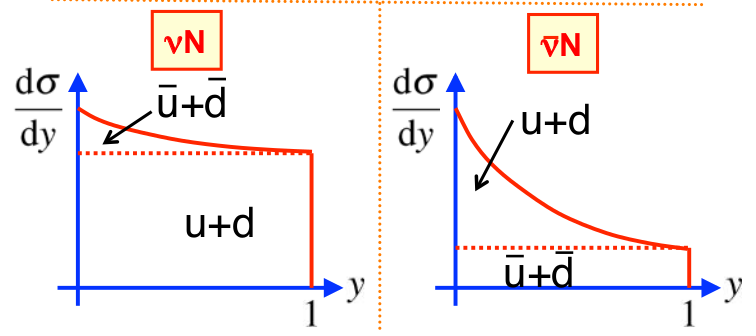
\includegraphics[width=0.5\textwidth,valign=c]{figs/nudis.png}
    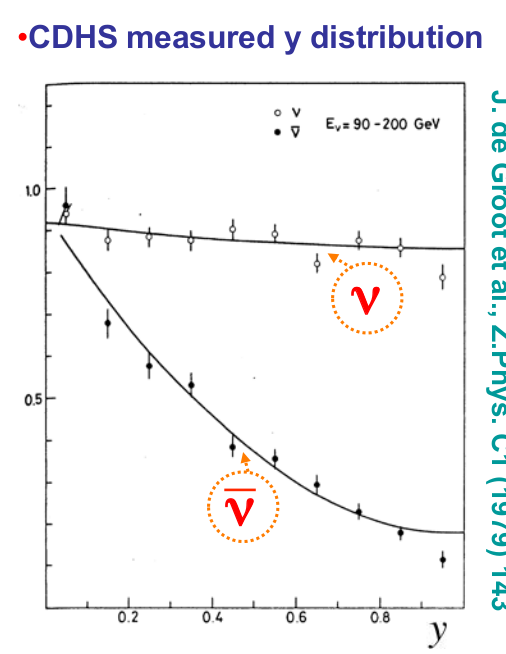
\includegraphics[width=0.3\textwidth,valign=c]{figs/cdhs.png}
  \end{center}
  \item First neutral current interactions were at Gargamelle
  \begin{itemize}
    \item Also a $\nu_\mu$ beam at a bubble chamber detector
    \item Both nucleon DIS and electron scattering were looked for (hadronic shower and free $\el$, respectively)
    \item Reject events with final-state $\mu$ \thus cannot be weak current
  \end{itemize}
\end{itemize}

\subsubsection{Weak contributions to $e$-$p$ scattering}
\begin{itemize}
  \item At high $Q^2$, CC scattering starts to be comparable to (or even dominate) NC (since $\alpha_W > \alpha$)
  \begin{itemize}
    \item Can be differentiated due to different final state: no final state lepton in CC
  \end{itemize}
  \item In general, $\el p$ scattering cross-section is higher than $\pos p$ scattering for two reasons:
  \begin{itemize}
    \item CC: $\el p$ scattering probes high $x$ part of $u_V$ pdf, while $\pos p$ probes $d_V$ pdf (and $u_V(x) > d_V(x)$)
    \begin{itemize}
      \item At low $Q^2$ this difference can be ignored and sea antiquark pdfs become significant
    \end{itemize}
    \item NC: there is $\gamma/Z$ interference at high $Q^2$ which is constructive for $\el p$ and destructive for $\pos p$
  \end{itemize}
\end{itemize}
\embedimgw{figs/weakdis.png}{.4}

\section{Neutrinos and oscillations}
\begin{itemize}
  \item We know that there are different flavors of neutrinos by searching for:
  \embedimgw{figs/mu2e.png}{.3}
  \begin{itemize}
    \item Experiment puts $\text{Br}(\mu\rightarrow\el\gamma)<10^{-11}$
  \end{itemize}
\end{itemize}

\subsection{Solar neutrinos}
\embedimgw{figs/solarnu.png}{.6}
\begin{itemize}
  \item Main source of $\nu_e$
  \item $pp$ reactions:
  \begin{gather*}
    p+p\rightarrow D + \pos +\nu_e \\
    D+p\rightarrow _2^3\text{He} + \gamma \\
    _2^3\text{He}+_2^3\text{He}\rightarrow _2^4\text{He}+p+p \numberthis
  \end{gather*}
  \begin{itemize}
    \item Binding energy of deuteron is only $2.2~\mev$ \thus $E_\nu < 0.5 ~\mev$
    \item Difficult to detect ($\sigma_{\nu N} \propto E_\nu$) so not used in experiments
  \end{itemize}
  \item $\beta$-decay of $^8\text{B}$
  \begin{gather*}
    ^4_2\text{He}+^3_2\text{He}\rightarrow_4^7\text{Be}+\gamma\\
    _4^7\text{Be}+p\rightarrow_5^8\text{B}+\gamma\\
    _5^8\text{B}\rightarrow_4^8\text{Be}^*+\pos+\nu_e\numberthis
  \end{gather*}
  \begin{itemize}
    \item Most used in experiments
    \item $E_\nu$ up to $15~\mev$
  \end{itemize}
  \item Electron capture: $^7\text{Be}+\el \rightarrow ^7\text{Li}+\nu_e$
  \begin{itemize}
    \item Two lines (corresponding to different electron excitations)
    \item Two discrete lines $<1~\mev$
  \end{itemize}
  \item $p+\el+p\rightarrow ^2\text{H}+\nu_e$
  \begin{itemize}
    \item Single line at $1.5~\mev$
  \end{itemize}
\end{itemize}
\subsubsection{Experimental detection}
\begin{itemize}
  \item Homestake
  \begin{itemize}
    \item Large vat of $\text{C}_2\text{Cl}_4$
    \item Flux was measured by counting number of $^{37}\text{Ar}$ atoms
    \item $\nu_e+\text{Cl}\rightarrow \text{Ar}+\el$
    \item Found the solar neutrino problem
    \begin{itemize}
      \item Expected was $1.7$ interactions per day
      \item Found $.5$ interactions per day
    \end{itemize}
  \end{itemize}
  \item Super-Kamiokande
  \begin{itemize}
    \item $50$ kt water Cerenkov detector surrounded by $11$k PMTs
    \item Counts $\nu_e\el\rightarrow\nu_e\el$ events (two leading-order $t$-channel diagrams involving $W$ and $Z$)
    \begin{itemize}
      \item Stability of oxygen nucleus limits CC interaction with oxygen nucleons at low (solar neutrino) energies
    \end{itemize}
    \item Signature is ring of light
    \begin{itemize}
      \item $\el$ is stopped in chamber, so $N_\gamma \propto E_e$
      \item Can discriminate muons (from atmospheric neutrinos) due to sharper ring ($\el$ diffuse more). Muons only arise from NC interactions
    \end{itemize}
    \item Below $E_\nu < 5~\mev$, radioisotope $\beta$-decay backgrounds dominate
    \item Confirms solar neutrino deficit $\sim1/2$ of expected flux
  \end{itemize}
  \item SNO
  \begin{itemize}
    \item Designed to detect electron neutrinos as well as total neutrino flux
    \item Charged current
    \begin{itemize}
      \item $\nu_e +D(pn) \rightarrow \el+p+p$
      \item $\nu_e+\el \rightarrow \nu_e+\el$ (also a NC diagram for this)
      \item Only $\nu_e$ participates because neutrino energies are not high enough to produce $\mu,\tau$
    \end{itemize}
    \item Neutral current
    \begin{itemize}
      \item $\nu_\ell+D(pn)\rightarrow \nu_\ell+p+n$
      \item $\nu_\ell + \el \rightarrow \nu_\ell+\el$
      \item All three flavors participate
    \end{itemize}
    \item Can measure total flux using all processes. Nucleon scattering has higher cross-sections
    \begin{itemize}
      \item Use elastic scattering off electrons to determine fraction of flux that comes from the sun ($\el$ direction is correlated with $\nu$ direction)
    \end{itemize}
    \item Results
    \begin{itemize}
      \item Again, confirms solar neutrino deficit
      \item On the other hand, found that the \emph{total} neutrino flux from the Sun is equal to predicted $\nu_e$ flux \thus first indication of oscillations
    \end{itemize}
  \end{itemize}
\end{itemize}

\subsection{Mass and weak eigenstates}
\begin{itemize}
  \item No reason to expect mass and weak eigenstates of neutrinos to be the same
  \item Mass eigenstates are the physical particle states
  \begin{itemize}
    \item i.e. satisfy $i \partial_t\nu_k = E\nu_k$ for $k=1,2,3$
  \end{itemize}
  \item So a Feynman diagram with an internal $\nu_\ell$ line is really the coherent addition of three diagrams with internal $\nu_k$ lines. If $k=1,2,3$: 
  \embedimgw{figs/internalnulines.png}{.6}
  \item Can define the $\nu_\ell$ states as linear combinations of the particle states:
  \begin{equation}
    |\nu_\ell\ra = \sum_{k=1,2,3} U^*_{\ell k} |\nu_k\ra
  \end{equation}
  \item The $W$ interaction vertex consequently must be written in terms of the mass eigenstates:
  \begin{equation}
    \left(-i U_{\ell k} \frac{g_W}{\sqrt{2}}\right) \bar\ell \gamma^\mu \frac{1}{2} (1-\gamma^5) \nu_k
  \end{equation}
  \begin{itemize}
    \item For interactions involving an outgoing $\nu$ or incoming $\nubar$, $U^*$ is in the vertex factor (i.e. the spinor is in the adjoint rep)
    \item If there is an incoming $\nu$ or outgoing $\nubar$, the spinor is in the fund. rep and $U$ is used
  \end{itemize}
\end{itemize}

\subsubsection{Example: oscillation between two flavors}

\noindent Here is the full derivation for oscillation between two flavors. Suppose there are two flavors $e,\mu$ and two mass eigenstates $1,2$. The free-particle states of the latter propagate as:
\begin{gather}
  |\nu_k(t)\ra = |\nu_k\ra e^{-i p_k\cdot x}
\end{gather}
where $p_k = (E_k,\p_k)$. Let us parametrize $U$ by an angle $\theta$:
\begin{equation}
  \begin{pmatrix} \nu_e \\ \nu_\mu \end{pmatrix} = 
  \begin{pmatrix} \cos \theta & \sin\theta \\ -\sin\theta & \cos\theta \end{pmatrix}
  \begin{pmatrix} \nu_1 \\ \nu_2 \end{pmatrix} 
\end{equation}
Suppose $\nu_e$  is produced at $t=0$:
\begin{equation}
  |\nu(0)\ra = |\nu_e \ra = \cos\theta|\nu_1\ra + \sin\theta|\nu_2\ra
\end{equation}
The evolution is then given by the free particle equation above:
\begin{equation}
  |\nu(x)\ra = \cos\theta |\nu_1\ra e^{-ip_1\cdot x} + \sin\theta |\nu_2\ra e^{-ip_2\cdot x}
\end{equation}
Now suppose the neutrino interacts weakly at a distance $L$ and time $T$. It will be projected into a weak eigenstate. At this point, the wavefunction is:
\begin{equation}
  |\nu(T,L)\ra = \cos\theta |\nu_1\ra e^{-i\phi_1} + \sin\theta |\nu_2\ra e^{-i\phi_2}, \quad \phi_k = E_k T - p_k L
\end{equation}
If we invert $U$ and plug into the above equation:
\begin{align*}
  |\nu(T,L)\ra &= \cos\theta e^{-i\phi_1}\left[\cos\theta |\nu_e\ra - \sin\theta|\nu_\mu\ra\right] + \sin\theta e^{-i\phi_2}\left[\sin\theta |\nu_e\ra + \cos\theta|\nu_\mu\ra\right]\\
  &= e^{-i\phi_1} \left( \left[\cos^2\theta+ e^{i\Delta\phi_{12}}\sin^2\theta\right]|\nu_e\ra + \left[1-e^{i\Delta\phi_{12}}\right]\sin\theta\cos\theta|\nu_\mu\ra \right) \numberthis
\end{align*}
where
\begin{equation}
  \Delta\phi_{12} = \phi_1 - \phi_2
\end{equation}
If $\Delta\phi_{12} \neq 0$, the $\nu_\mu$ projection is non-zero. Squaring the factor multiplying $|\nu_\mu\ra$, we get:
\begin{equation}
  P(\nu_e\rightarrow \nu_\mu) = \sin^2(2\theta) \sin^2 \left(\frac{\Delta\phi_{12}}{2}\right)
\end{equation}
There are different assumptions one could make in calculating $\Delta\phi_{12}$ (in principle, one should evolve wavepackets instead of free particles). Here we assume $p_1 = p_2$, but one could also assume $E_1 = E_2$ or $\beta_1 = \beta_2$ and get the same answer.
\begin{align*}
  \Delta\phi_{12} &= (E_1-E_2)T - (p-p)L = \left[\sqrt{p^2+m_1^2} - \sqrt{p^2+m_2^2}\right]T\\
    &\approx \left[p \left(1+ \frac{m_1^2}{2p^2}\right) - p \left(1+ \frac{m_1^2}{2p^2}\right)\right]T\\
    &= \left(m_1^2-m_2^2\right) \frac{L}{2p} \equiv \Delta m^2_{12} \frac{L}{2E_\nu} \numberthis
\end{align*}
In the last line, we assume $\beta \approx 1$ and $p\approx E_\nu$. 

\subsubsection{Oscillation between three flavors}
\begin{itemize}
  \item The calculation is similar to above, but more complicated
  \begin{itemize}
    \item Have to deal with the fact that things like $e\rightarrow\mu\rightarrow \tau$ can happen, affecting the oscillation probabilities
  \end{itemize}
  \item The matrix is known as the PMNS matrix
  \item The phase differences are defined as:
  \begin{equation}
    \Delta_{ij} = (m_i^2-m_j^2) \frac{L}{4E_\nu} \equiv \Delta m_{ij}^2 \frac{L}{4E_\nu}
  \end{equation}
  Note tat they are not all independent. We can write $\Delta_{31} = \Delta_{32} + \Delta_{21}$
  \item The survival probability is:
  \begin{equation}
    P(\nu_e\rightarrow\nu_e) = 1 - 4|U_{e1}|^2|U_{e2}|^2 \sin^2\Delta_{21} - 4|U_{e1}|^2|U_{e3}|^2 \sin^2\Delta_{31} - 4|U_{e2}|^2|U_{e3}|^2 \sin^2\Delta_{32}
  \end{equation}
\end{itemize}

\subsubsection{Neutrino masses}
\begin{itemize}
  \item Neutrino oscillation experiments are only sensitive to \emph{difference} in squared masses, not the masses themselves
  \item Looking at end-point of electron $Q$ distribution in tritium $\beta$-decay shows that the lightest eigenstate must be $\lesssim 2~\ev$
  \item Large-scale structure and measurement of C$\nu$B limit $\sum_k m_{k} \lesssim 1~\ev$
  \item Best measurements of mass differences are:
  \begin{gather*}
    \Delta m_{21}^2 \sim 10^-4~\ev^2\\
    \Delta m_{32}^2 \sim 10^-3~\ev^2\numberthis
  \end{gather*}
  \begin{itemize}
    \item The sign of $\Delta m_{32}^2$ is unknown. $m_3>m_2$ is the normal hierarchy; the inverse is the inverted hierarchy.
    \embedimgw{figs/nuhierarchy.png}{.6}
    \item $\Delta m_{31}^2$ has not been measured independently.
  \end{itemize}
\end{itemize}

\subsubsection{CP violation}
\begin{itemize}
  \item Recall that QED and QCD conserve $C$ and $P$ separately, so they cannot lead to $CP$ violation. Weak interactions could be a source of $CP$ violation.
  \item Two ways of determining if $CP$ violation occurs in the PMNS matrix:
  \begin{itemize}
    \item Measure $P(\nu_e\rightarrow\nu_\mu)$ and the $CP$-transformed quantity $P(\nubar_e\rightarrow\nubar_\mu)$ (note $C$ is not enough since you would go from LH $\nu$s to RH $\nubar$s). Measure the difference in the probabilities; it should be $0$ if $CP$ is not violated
    \item Assuming $CPT$ invariance, $CP$ violation implies $T$ violation. Therefore, one could measure $P(\nu_\mu\rightarrow \nu_e)$ and check it is equal to $P(\nu_e\rightarrow\nu_\mu)$
  \end{itemize}
  \item In order for this to occur, elements of the PMNS matrix must have imaginary components. There is in fact only one independent complex phase in the matrix (the others can be absorbed into particle definitions):
  \begin{equation}
    \begin{pmatrix} 
      U_{e1} & U_{e2} & U_{e3} \\
      U_{\mu1} & U_{\mu2} & U_{\mu3} \\
      U_{\mu1} & U_{\mu2} & U_{\tau3} 
    \end{pmatrix} = 
    \begin{pmatrix} 
      c_{12}c_{13} & s_{12}s_{13} & s_{13}e^{-i\delta} \\
      -s_{12}c_{23}-c_{12}s_{23}s_{13}e^{i\delta} & c_{12}c_{23}-s_{12}s_{23}s_{13}e^{i\delta} & s_{23}c_{13}\\
      -s_{12}s_{23}-c_{12}c_{23}s_{13}e^{i\delta} & c_{12}s_{23}-s_{12}c_{23}s_{13}e^{i\delta} & c_{23}c_{13}
    \end{pmatrix}   
  \end{equation}
  \item Current experiments are not sensitive to $CP$ violation in the neutrino sector
\end{itemize}

\section{Oscillation experiments}
\begin{itemize}
  \item Both neutrinos and antineutrinos have $t$-channel CC and NC interactions with electrons and nucleons
  \begin{itemize}
    \item Antineutrinos also have a $s$-channel CC interaction $\nubar_e \el \rightarrow \nubar_e \el$
  \end{itemize}
  \item Muon neutrinos interact with electrons through CC only if $E_{\nu_\mu}>11~\gev$ (need to be able to create the muon). Threshold for taus is $3~\tev$
\end{itemize}

\subsection{Reactor experiments}
\begin{itemize}
  \item Use $\nubar_e$ flux from $\beta^-$ decays of $^{235}\text{U},~^{238}\text{U},~^{239}\text{Pu},~^{241}\text{Pu}$
  \begin{itemize}
    \item Flux is precisely known from power output of reactor
    \item Energies are $\sim\mev$, so nucleon CC interaction is inverse $\beta$ decay (as opposed to DIS)
  \end{itemize}
  \item Because energies are too low to produce $\mu,\tau$ in either nucleon or electron interactions, oscillation is observed through deficit of $\nubar_e$
  \item Two oscillation wavelengths
  \begin{itemize}
    \item Long-wavelength: sensitive to $\Delta m_{21}^2,\theta_{12}$. This is what solar neutrino experiments are sensitive to. $\ord{100}$ km
    \item Short-wavelength: sensitive to $\Delta m_{32}^2,\theta_{13}$. $\ord1$ km
  \end{itemize}
\end{itemize}
\embedimgw{figs/nue_probability.png}{.5}

\subsubsection{Short baseline}
\begin{itemize}
  \item Sensitive to only short-wavelength oscillations
  \begin{equation}
    P(\nubar_e\rightarrow \nubar_e) \approx 1- \sin^2(2\theta_{13}) \sin^2 \left(\frac{\Delta m_{32}^2 L}{4E_\nubar}\right)
  \end{equation}
  \item Daya Bay
  \begin{itemize}
    \item Detectors positioned at various distances from reactor cores ($470, 580, 1650$ m away)
    \item Detector is liquid scintillator loaded with Gd, surrounded by PMTs
    \item Inverse $\beta$-decay has highest cross-section ($\nubar_e+p\rightarrow \pos+n$)
    \item Signal signature
    \begin{itemize}
      \item $\pos$ annihilates with an $\el$ and releases two prompt photons
      \item Low energy $n$ drifts for a while until capture by a Gd nucleus, which then de-excites and releases a photon (timescale of $100~\mus$)
    \end{itemize}
    \item Assuming known value of $\Delta m_{32}^2$, Daya Bay measures:
    \begin{equation}
      \sin^2(2\theta_{13}) = 0.10 \pm 0.01
    \end{equation}
  \end{itemize}
  \item KamLAND
  \begin{itemize}
    \item Scintillator-PMT detector at 130-240 km away from reactor core
    \item Again, I$\beta$D is dominant process
    \item Signal signature
    \begin{itemize}
      \item Two prompt photons from $\pos$ annihilation
      \item Delayed $2.2~\mev$ photon from $n+p\rightarrow D+\gamma$
    \end{itemize}
    \item Measured $\Delta m_{21}^2\sim 8\times 10^{-5}~\ev^2$ and $\sin^2(2\theta_{12})=0.87$
  \end{itemize}
\end{itemize}

\subsubsection{Long baseline}
\begin{itemize}
  \item Relies on accelerator-based neutrino beams
  \item Use one near and one far detector. Systematic uncertainties will be the same, so can assume they cancel in the ratio when measuring survival probabilities
  \item MINOS
  \begin{itemize}
    \item High intensity $\nu_\mu$ beam from Fermilab
    \begin{itemize}
      \item $E_\nu \sim 1\text{-}5~\gev$
      \item $L=735$ km
    \end{itemize}
    \item Dominant interaction is $\nu_\mu N\rightarrow\mu^-+$hadrons
    \item Detector is planes of iron with plastic scintillator inbetween
    \begin{itemize}
      \item Magnetic field to curve charge particles
      \item Muon is identified and $p_\mu$ is measured by looking for a long curved track (hadrons will be stopped quickly)
      \item $E_\text{had}$ is measured by amount of scintillation light near beginning of muon track (interaction vertex)
    \end{itemize}
    \item At these energies, the oscillation associated with $\Delta_{21}$ is much longer than $L$ so can be ignored. Since $\theta_{13}$ is tiny, only $\mu,\tau$ need to be considered
    \item $\nu_\tau$ energies are too low to produce a $\tau$, so oscillation is measured by looking for a deficit of $\nu_\mu$ interactions
    \item Measures $|\Delta m_{32}^2| = 2.3 \times 10^{-3}~\ev^2$ and $\sin^2(2\theta_{23})\gtrsim 0.9$
  \end{itemize}
\end{itemize}

\subsubsection{Global picture}
\begin{itemize}
  \item Mass differences measured to within $5\%$:
  \begin{itemize}
    \item $\Delta m_{21}^2 = 7.6 \times 10^{-5}~\ev^2$
    \item $\Delta m_{32}^2 = 2.3 \times 10^{-3}~\ev^2$
  \end{itemize}
  \item Three of the four PMNS parameters are measured (or are constrained):
  \begin{itemize}
    \item $\sin^2(2\theta_{12}) = 0.87$
    \item $\sin^2(2\theta_{23}) > 0.92$
    \item $\sin^2(2\theta_{13}) > 0.10$
  \end{itemize}
  \item The CP violating phase $\delta$ is not constrained at all
\end{itemize}


\begin{appendices}
\section{Bibliography}

\vspace{5mm}

\noindent Universitat Heidelberg, \emph{Solar neutrino problem}. \url{http://www.kip.uni-heidelberg.de/tt_detektoren/neutrinos.php?lang=en}

\vspace{5mm}

\noindent Tapper A., \emph{High $Q^2$ neutral current cross sections in $\el p$ DIS}. \url{http://www.hep.ph.imperial.ac.uk/~tapper/talks/dis04.pdf}

\vspace{5mm}

\noindent Thomson M., \emph{Modern Particle Physics} and online lecture notes (\url{http://www.hep.phy.cam.ac.uk/~thomson/partIIIparticles/welcome.html})
\vspace{5mm}

\noindent Klute M., Lecture notes from 8.811

\end{appendices}

\end{document}
